\subsection{Initial Model Evaluation}
\label{init_eval}

\begin{table*}[t]
\begin{tabular}{|l|c|c|c|l|}
\hline
 Name  & Processor  &  Cache &  Offchip BW & Description \\ \hline
 p+c+b+ & benefits & benefits & benefits &  Copies data from many large blocks, with intra-block reuse (multithreaded)\\ \hline
p--c+b+ & oblivious & benefits & benefits &  Copies data from many large blocks, with intra-block reuse (single threaded)\\ \hline
p+c--b+ & benefits & oblivious & benefits &  Streaming copies with no reuse (multithreaded)\\ \hline
p--c--b+ & oblivious & oblivious & benefits &  Streaming copy with no reuse (single threaded)\\ \hline
p+c+b-- & benefits & benefits & oblivious &  Copies data repeatedly from single large blocks (multithreaded)\\ \hline
p--c+b-- & oblivious & benefits & oblivious &  Copies data repeatedly from a single large block (single threaded)\\ \hline
p+c--b-- & benefits & oblivious & oblivious &  Pointer chases through long lists (multithreaded)\\ \hline
p--c--b-- & oblivious & oblivious & oblivious &  Pointer chases through a long list (single threaded)\\ \hline
\end{tabular}
\caption{Synthetic microbenchmark descriptions. Each benchmark captures a different combination of responses to resource allocations.  ``Benefits'' means that application performance improves as more of that resource is allocated to it (though sometimes only up to a point).  ``Oblivious'' means that the application performance barely improves or does not improve at all as more of that resource is allocated to it.}
\label{table:benchmarks}
\end{table*}

\begin{table*}[t]
\footnotesize
\begin{tabular}{|c|c|l|l|}
\hline
 Phase  & Name & Description & Behavior \\ \hline 
 1 & Cluster  & Observation probability computation, step 1 &  Accumulate, up to 6 MB data read, 800KB written\\ \hline
 2 & Gaussian  & Observation probability computation, step 2 &  Calculate, up to 800KB read, 40KB written\\ \hline
 3 & Update & Non-epsilon arc transitions &40KB read, small blocks, dependent on graph connectivity\\ \hline
 4 & Pruning & Pruning states & Small blocks, dependent on graph connectivity\\ \hline
 5 & Epsilon & Epsilon arc transitions & Small blocks, dependent on graph connectivity\\ \hline
\end{tabular}
\caption{Description of phase behavior in LVSCR application.}
\label{table:app}
\end{table*}

\subsubsection*{Model Inputs and Outputs}
Our models use allocations of machine resources as independent variables (i.e. inputs) and some metric of application performance as the dependent variables (i.e. outputs).  The inputs we include in this study are number of cores, off-chip bandwidth allocation, L2 cache ways and L2 cache banks.  Since all input parameters are actually allocation sizes (i.e. integers), they are easily represented as terms in the regression analysis.

We use cycles of execution time as a predicted output representative of application performance.  To help correlate application performance with resource utilization and not just resource allocation we also collect data from several performance counters that are usually strongly correlated with performance. These utilization metrics include L2 cache misses, L2 cache requests, and instructions retired. Any metric of interest that is measurable at runtime can be a potential output candidate. All of these models can be referenced by the spatial resource scheduling algorithm.

%%A final model we create predicts the energy consumed by a resource allocation, whice is useful  for energy-aware scheduling decisions. We calculate the energy used by each allocation by creating a simple energy model which incorporates energy levels for allocated versus unallocated resources and uses performance counter data as a proxy for resource activity.  Such an energy model is clearly somewhat simplistic --- we include it to show that our scheduling framework can feasibly make decisions based on per allocation energy if that data is a given input.  We use a simplified version of some of the activity based energy models in previous work \cite{}.  

\subsubsection{Partitioning Mechanisms}
To achieve performance isolation for each application and improve model accuracy, we implement hardware partitioning mechanisms on several of the most important shared on--chip  resources. Shared resources include discrete functional units (e.g. cores), containers with shared capacity (e.g. caches), or communication media with shared bandwidth (e.g. interconnects).  There may be many such resources on an individual chip and even more in an entire computer system. In this study, we provide partitioning mechanisms for cores, L2 cache capacity, and interconnect bandwidth to DRAM. 
 The following subsections describe these partitioning mechanisms in greater detail.
 
 %Much prior work has been done to create hardware mechanisms in support of physical resource partitioning \cite{876484,967444,1194855,1086328,605420,1152161,1331730, 1241608,1382130,1250671,1194858,1275005,1088154,1318096,1399982,1399973, 1069998}.   

\subsubsection*{Core Pinning}
To partition cores, our implementation uses the thread affinity feature built into the Linux 2.6 kernel.  We restrict the threads belonging to an application to run on the cores assigned to that application.  For now we assume a homogeneous collection of cores, and that only last level caches are shared among applications, which means that there is nothing to differentiate a core from any other when they are being allocated. 
%In the future we anticipate moving to a system with two-level scheduling where user-level code schedules the threads on the cores allocated in a partition like the system described in \cite{citation222}.

\subsubsection*{Globally Synchronized Frames}
To partition off-chip bandwidth, we use the Globally Synchronized Frames (GSF) approach presented in Lee et al. \cite{1382130}.  We choose this approach because it does not require complex hardware modifications, provides strict QoS guarantees for minimum bandwidth and the maximum delay of the network, and provides proportional sharing of excess bandwidth.  GSF controls the number of packets that a core can inject into the network per frame, and each core is guaranteed to get the number of packets allocated to it each frame.  GSF enables cores to inject packets into future frames if their current allocation is already exceeded.  This allows excess bandwidth to be shared among cores proportional to their packet allocation.  To simplify prediction by making performance more deterministic, our current implementation does not make any future frames available during training, meaning that applications get exactly their allocation each frame.

\subsubsection*{Cache Partitioning}
Many cache partitioning mechanisms previously studied have used some form of way-based partitioning \cite{1331730,1152161,605420,1250671,1194855,1086328,1399982}.  While way-based partitioning is relatively easy to implement in hardware, it is by necessity relatively coarse-grained since it is limited by the number of ways in the cache.  Partitioning among ways can cause significant performance degradation in many applications due to the decreased associativity available to each partition. 

Way-based partitioning keeps the cache access logic simple since data will still always reside in the same set, regardless of current partition.  However, in the case of manycore architectures, this access simplicity will be less important since large shared caches are likely to be distributed in multiple banks.  Accessing a non-local cache bank will require a request to be sent across an interconnect. We argue that this extra communication step introduces the potential for a level of indirection in the cache indexing policy, and the added flexibility can be used to allow different banks to be assigned to different applications. This approach can be particularly advantageous in a NUCA system so that applications can be assigned cache banks nearest to their cores. Rather than sending the request to the bank identified by the address index, we can instead use the mapping of banks to applications to determine which cache bank should be the target of the incoming request. 

The major overhead of this technique comes when a bank is allocated to a new application -- for the sake of the coherence policy, the system must copy back all dirty data in that bank before changing the routing used for cache requests.  We allow both bank-based and way-based partitioning of cache capacity in our implementation, though the experiments here use only bank-based partitioning to preserve cache associativity.



\subsubsection*{Modeling Techniques}
We use multivariate regression techniques to create explicit statistical models for predicting the performance of an application given a resource allocation of a particular size.  We create one regression model per performance metric per application phase. 
 
Linear least-squares regression techniques produce simple models that can be expressed concisely and are therefore more portable. Linear regression techniques can outperform nonlinear ones when training sets are small, the data has a low signal to noise ratio, or sparse sampling is used\cite{hastie}. These criteria apply in our case. These models are attractive due to their simplicity, but their restricted expressiveness may reduce their accuracy of the underlying system.

Linear models may be realized in varying forms (i.e. it is the combination of terms that is linear, rather than the degree of each term).  The simplest models are linear additive models, which take the form:

\begin {equation}
y(x) = a_0 + \sum_{i=1}^{N}{a_ix_i} 
\end {equation}

Multivariate linear additive models contain one term for each variable (i.e. an allocation, $x_i$) and an intercept term ($a_0$).  The regression tunes the coefficient associated with each term ($a_i$) to fit the sample data as accurately as possible.  Note that the linear additive model has no way to represent any possible interaction between the variables, implying that all variables are independent---which is expressly not true in our scheduling scenario.  We include them in our study as a straightforward baseline for comparison.
%For example, a smaller cache size will result in increased cache misses and an increased demand for memory bandwidth, meaning that the effect of a change in bandwidth allocation is not independent from a change in cache size in terms of its effect on performance.  

More complex multivariate linear regression models often include terms for variable interaction and polynomial terms of degree 2 or more.  Such models are commonly termed {\em response surface models} and have the general form:

\begin {equation}
y(x) = a_0 + \sum_{i=1}^{N}{a_ix_i} + \sum_{i = 1}^{N}\sum_{j=i}^{N}{a_{ij}x_ix_j} + ...
% \sum_{i=0}^{N}{a_{ii}x_i^2}
\end {equation}

These polynomial models capture more complex dependencies between the input variables.  However, we as modelers are still expressing beliefs about the nature of the relationship between input and output in the form we give the polynomial equation.  

Selecting the best possible equation form for the data automatically requires the use of nonlinear regression techniques such as local regression, cubic splines, neural networks, or genetic programming \cite{alvarez-thesis, bodik-acdc09, wasserman-book}.  The disadvantage of these techniques is that the models may create difficulties for analytic maximization algorithms. 
%LOESS models have been used in the past in situations where the models must be retrained online as more data points are collected from the running system \cite{bodik-acdc09}. 

Genetic programming is a technique, based on evolutionary biology, used to optimize a population of computer programs according to their ability to perform a computational task. In our case, the `program' is an analytic equation whose evaluation embodies a response surface model, and the `task' is to match sample data points obtained from full--scale simulations \cite{alvarez-thesis}. The output, termed a
{\em genetically programmed response surface} (GPRS), are nonlinear models that create explicit equations describing the relationship between design variables and performance, and we incorporate them into our framework as an example of a nonlinear modeling alternative.
A GPRS is generated automatically, meaning that the modeler does not have to specify the form of the response surface equation in advance. Instead, genetic programming \cite{koza} is used to create an equation and tune the coefficients.  For more information on GPRS creation, see \cite{alvarez-thesis} or \cite{cook-dac08}.

Other statistical machine learning techniques such as clustering might also be used in our framework to make predictions about application behavior.  Any such technique must be able to correlate changes in resource allocations to changes in performance in an application--specific way.  Ganapathi et al. have had success using machine learning to model application performance and select the best performing configuration in \cite{Archana}. Investigating more complicated models is a subject of our future work.


In this section we evaluate the accuracy of the different modeling techniques and their effectiveness as inputs to an algorithm that assigns spatial allocations to applications.

\subsubsection*{Experimental Testbed}
We use Virtutech Simics \cite{simics} to simulate a CMP system with a two level on-chip memory hierarchy to collect the data used create our performance models and to test the effectiveness of our resource scheduling framework.  Simics is a full system simulator capable of running a commodity OS and completing simulations consisting of billions of cycles. We modify the Simics cache and memory timing modules to reflect the capabilities of our hardware partitioning mechanisms.  Our target machine has 10 cores, private 64KB L1D and 32KB L1I caches for each core and a shared L2 (16 MB, 16-way set associative).  All caches have 128 B lines.   All banks in the L2 cache have uniform access time of 7 cycles.  Our target machine runs Fedora Core 5 Linux (kernel 2.6.15). We constrain the simulated system to a maximum allocation of 10 cores, 16 MB of L2 cache, and 4 cache lines/cycle of off-chip bandwidth, and a minimum allocation of 1 core, 16 KB of L2 cache, and 5 cache lines/thousand cycles of off-chip bandwidth. 

\subsubsection*{Benchmarks}
We created a set of synthetic microbenchmarks specifically designed to evaluate our modeling techniques and spatial scheduling algorithm by creating clear contrasts between different allocation decisions.  Table \ref{table:benchmarks} describes these benchmarks.  In general, each benchmark represents a generic category of behavior that we might expect to see in phases of real applications.  We classify the benchmarks based on whether they benefit from additional processor, cache or bandwidth resources, or whether they derive no benefit from running on a large allocation of a given resource.  We also limit the size of the benchmarks along these resource dimensions such that they will encounter performance cliffs on our simulated machine.  For example, a benchmark's performance might benefit from additional cores up to 4 cores but not from more than 4 cores.   Some benchmarks are parallelized with {\tt pthreads} \cite{pthreads}.  The benchmarks each execute an average of 1.9 billion cycles per sample point.

We also evaluate a real multithreaded application with multiple phases of behavior, specifically 
a Hidden-Markov-Model (HMM) based inference algorithm that is part of a large-vocabulary continuous-speech-recognition (LVCSR) application \cite{chong-eama08, huang-speech}. This application case study demonstrates the varying ability of our models to capture real application behavior.

LVCSR applications analyze a set of audio waveforms and attempt to distinguish and interpret the human utterances contained within them. The recognition network we use here models a vocabulary of over 60,000 words and consists of millions of states and arcs. The inference process is divided into a series of five phases, and the algorithm iterates through the sequence of phases repeatedly with one iteration for each input frame. Table~\ref{table:app} lists the characteristics of each phase of the application.  Each phase runs for an average of 24 billion cycles for each sample point. 

\begin{figure*}
	\centering
	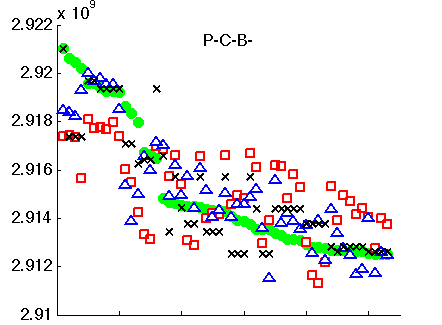
\includegraphics[scale = 0.34] {ooo_trainpredplot.png} 
	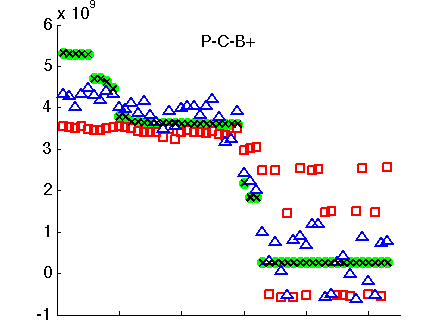
\includegraphics[scale = 0.34] {oop_trainpredplot.png}
	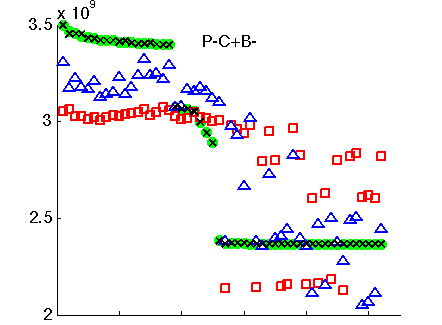
\includegraphics[scale = 0.34] {opo_trainpredplot.png} 
	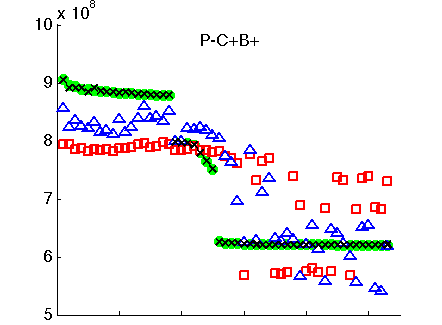
\includegraphics[scale = 0.34] {opp_trainpredplot.png}
	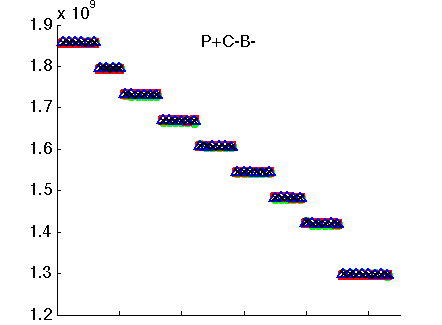
\includegraphics[scale = 0.34] {poo_trainpredplot.png} 
	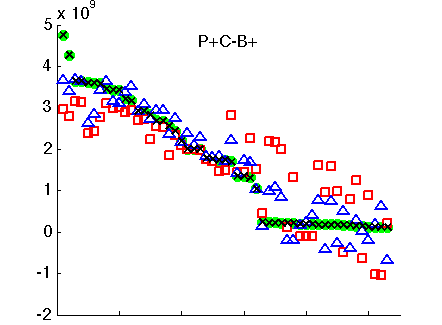
\includegraphics[scale = 0.34] {pop_trainpredplot.png}
	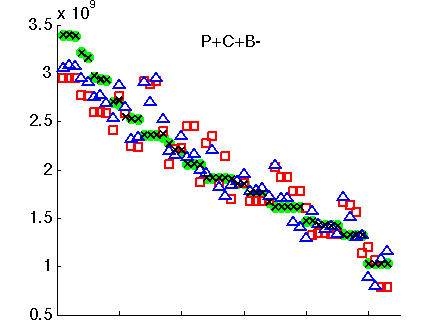
\includegraphics[scale = 0.34] {ppo_trainpredplot.png} 
	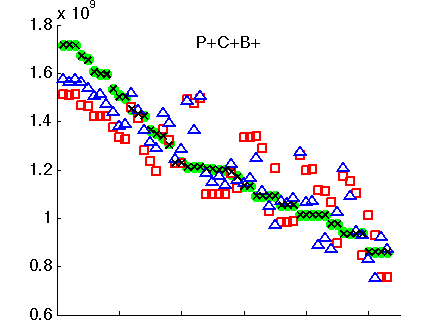
\includegraphics[scale = 0.34] {ppp_trainpredplot.png} \\
	
\includegraphics[scale = 0.5] {acc_comp_legend_horz.png} 
	\caption{ \small Comparison of model accuracy for the eight microbenchmarks when predicting runtime in cycles. Each point represents a prediction for a machine configuration, and points are ordered along the x-axis based on decreasing measured run time. Y-axis plots predicted or measured runtime in cycles; note the differing ranges. In most cases, the nonlinear GPRS--based model is so accurate that it precisely captures all sample points.}
	\label{fig:acc}
\end{figure*}

%%\subsection{Partitioning Mechanism Efficacy}       
%%It is worth noting that conflicts between different applications will always be destructive to performance and predictability.  The only danger to performance presented by hardware partitioning is the possibility of resource fragmentation, in which an application is allocated more of a resource than it can actually use.  However, a conservative allocation policy combined with fair sharing of excess resources can significantly mitigate this problem.

\subsubsection*{Evaluation of Model Accuracy}
In this section we examine the accuracy afforded by both the different linear regression models and the nonlinear GPRS--based regression model.  We choose a sample of 55 points from the space of 19200 possible allocations (or 0.3\%), and we train the models using this sample set.  The sample points were chosen using an Audze-Eglais DOE. 

We evaluate the accuracy of the model relative to measured performance on a set of points disjoint from the sample set.  Due to the length of our simulations, we cannot exhaustively compare to all possible allocations and so limit our model error analysis to a testing set of 10 randomly selected points.  We perform this analysis for several performance metrics captured from simulation, including runtime in cycles, number of instructions committed, number of cache accesses, and number of off-chip memory accesses.  

 Figure~\ref{fig:acc} plots the predictions versus measured data of a single performance metric for the sample set. While linear and nonlinear models perform equally well for some benchmarks, the nonlinear model is significantly more accurate at predicting others. The linear models struggle to capture the performance cliffs inherent to some benchmarks, especially those which move between being cache size-limited and bandwidth-limited.  In particular benchmarks which encounter a cliff and then saturate (such as the working set fitting in cache) are not faithfully modeled by the linear models.  The nonlinear model has no such difficulty.  It is also worth noting that the amount of error introduced in the linear additive and quadratic model causes them to predict negative values for some benchmarks.

\begin{table}
\small
\begin{tabular}{|l|c|c|c|}
\hline
Name & Additive & Quadratic & GPRS \\ \hline
 p--c--b-- & 0.06\% (0.04) & 0.04\% (0.04) &0.02\% (0.02) \\ \hline
 p--c--b+ &   234.07\% (287.44) & 139.21\% (167.10) &  0.23\% (0.40)   \\ \hline
 p--c+b-- &  12.67\% (5.30) &  8.26\% (5.30) &  0.02\% (0.02) \\ \hline
 p--c+b+ &  12.04\% (5.09) &  7.83\% (4.69) & 0.06\% (0.06)  \\ \hline
 p+c--b-- &  0.07\% (0.05) &  0.05\% (0.06)  &  0.05\% (0.03)  \\ \hline
 p+c--b+ &  271.05\% (377.53) & 164.23\% (226.23) & 0.51\% (1.08) \\ \hline
 p+c+b--&  13.08\% (6.91) & 8.79\% (7.32) & 0.06\% (0.07) \\ \hline
 p+c+b+&  12.07\% (4.86) &  8.05\% (5.49) & 0.08\% (0.06)  \\ \hline 
   \end{tabular}
 \caption{Means (standard deviations) of percentage error in runtime cycles for each of the predictive models for each of the microbenchmarks.}
\label{table:acc-cycles}
\end{table}

\begin{table}
\small
\begin{tabular}{|l|c|c|c|}
\hline
Name & Additive & Quadratic & GPRS \\ \hline
 cluster &  4.27\% (3.66) & 6.90\% (5.67)  & 15.52\% (10.36)  \\ \hline
 gaussian&  1.83\% (0.72) & 4.16\% (2.49) & 2.33\% (3.19)  \\ \hline
 update&  4.98\% (3.04) & 7.94\% (7.12)  & 5.89\% (5.09)  \\ \hline
 pruning&  2.27\% (1.08) & 10.70\% (10.29)  & 3.07\% (2.91)  \\ \hline
 epsilon &  3.88\% (4.01) & 4.66\% (4.27)  & 2.69\% (1.09)  \\ \hline  
   \end{tabular}
 \caption{Means (standard deviations) of percentage error in runtime cycles for each of the predictive models for each of the phases of the LVSRC application.}
\label{table:acc-cycles-lvsrc}
\end{table}
 
\begin{table}
\scriptsize
\begin{tabular}{|l|c|c|c|}
\hline
Name & Additive & Quadratic & GPRS \\ \hline
  p--c--b-- & 392.11\% (398.89) &  240.12\% (261.72) & 7.42\% (16.80)  \\ \hline
 p--c--b+ &  138133\% (290142)&  105682\% (248332) &  253.46\% (418.27)  \\ \hline
 p--c+b-- &   37225\% (65356) &  25797\% (47989) & 84.31\% (74.62)  \\ \hline
 p--c+b+ &   45276\% (82816) &  21819\% (30963) &  87.84\% (209.33)  \\ \hline
 p+c--b-- & 236.30\% (261.31) &  121.44\% (124.23) & 15.27\% (14.80)    \\ \hline
 p+c--b+ &   101696\% (169812)  &  73241\% (117426) & 25.42\% (31.95) \\ \hline
 p+c+b--&  16920\% (22871)&   12517\% (19362) & 7.47\% (8.25)  \\ \hline
 p+c+b+&   9480\% (11542) &  6647\% (9164) &  22.12\% (26.14)  \\ \hline 
  \end{tabular}
 \caption{Means (standard deviations) of percentage error in offchip accesses for each of the predictive models for each of the microbenchmarks.}
\label{table:acc-offchip}
\end{table}
 
\begin{table}
\small
\begin{tabular}{|l|c|c|c|}
\hline
Name & Additive & Quadratic & GPRS \\ \hline
 p--c--b-- & 0.03\% (0.04) & 0.03\% (0.05) & 0.28\% (0.36) \\ \hline
 p--c--b+ & 241.91\% (262.05)  & 218.93\% (382.43) &  0.1\% (0.07) \\ \hline
 p--c+b-- & 8.49\% (5.49) & 6.17\% (6.50) & 0.41\% (1.13) \\ \hline
 p--c+b+ & 8.01\% (5.2)  & 5.79\% (6.11) & 0.07\% (0.06) \\ \hline
 p+c--b-- & 7.28\% (10.50)  & 0.05\% (0.04) & 0.27\%(0.19) \\ \hline
 p+c--b+ & 233.26\% (250.1) & 153.10\% (234.34) &  4.89\% (12.97)\\ \hline
 p+c+b-- & 20.23\% (24.18)  & 5.10\% (4.26) &  0.30\% (0.28) \\ \hline
 p+c+b+ & 13.30\% (10.23)  & 5.25\% (4.77)  & 0.05\% (0.03) \\ \hline 
  \end{tabular}
 \caption{Means (standard deviations) of percentage error in cache transaction counts for each of the predictive models for each of the microbenchmarks.}
\label{table:acc-cache}
\end{table}

%\begin{table}
%\small
%\begin{tabular}{|l|c|c|c|}
%\hline
%Name & Cycles &Offchip Accesses &Cache Accesses \\ \hline
% p--c--b-- & 0.06\% (0.04) &  392.11\% (398.89) & 0.03\% (0.04) \\ \hline
% p--c--b+ &   234.07\% (287.44) & 138133\% (290142) & 241.91\% (262.05)  \\ \hline
% p--c+b-- &  12.67\% (5.30) & 37225\% (65356) & 8.49\% (5.49)  \\ \hline
% p--c+b+ &  12.04\% (5.09) &  45276\% (82816) & 8.01\% (5.2)  \\ \hline
% p+c--b-- &  0.07\% (0.05) &  236.30\% (261.31) & 7.28\% (10.50)  \\ \hline
% p+c--b+ &  271.05\% (377.53) & 101696\% (169812) & 233.26\% (250.1)  \\ \hline
% p+c+b--&  13.08\% (6.91) & 16920\% (22871) & 20.23\% (24.18)  \\ \hline
% p+c+b+&  12.07\% (4.86) &  9480\% (11542) & 13.30\% (10.23)  \\ \hline \hline
% cluster &  1 (1) & 1 (1)  & 1 (1)  \\ \hline
% gaussian&  1 (1) & 1 (1) & 1 (1)  \\ \hline
% update&  1 (1) & 1 (1)  & 1 (1)  \\ \hline
% pruning&  1 (1) & 1 (1)  & 1 (1)  \\ \hline
% epsilon &  1 (1) & 1 (1)  & 1 (1)  \\ \hline
% \end{tabular}
% \caption{Means (standard deviations) of percentage error for each of the performance measures for each of the benchmarks, as predicted by the linear response surface model.}
%\label{table:acc-lin}
%\end{table}
% 
%\begin{table}
%\small
%\begin{tabular}{|l|c|c|c|}
%\hline
%Name & Cycles &Offchip Accesses &Cache Accesses \\ \hline
% p--c--b-- & 0.04\% (0.04) &  240.12\% (261.72) & 0.03\% (0.05) \\ \hline
% p--c--b+ &  139.21\% (167.10) &  105682\% (248332) & 218.93\% (382.43)  \\ \hline
% p--c+b-- &  8.26\% (5.30) &  25797\% (47989) & 6.17\% (6.50)  \\ \hline
% p--c+b+ &  7.83\% (4.69) &  21819\% (30963) & 5.79\% (6.11)  \\ \hline
% p+c--b-- &  0.05\% (0.06) &  121.44\% (124.23) & 0.05\% (0.04)  \\ \hline
% p+c--b+ &  164.23\% (226.23) &  73241\% (117426) & 153.10\% (234.34)  \\ \hline
% p+c+b--&  8.79\% (7.32) &   12517\% (19362) & 5.10\% (4.26)   \\ \hline
% p+c+b+&  8.05\% (5.49) &  6647\% (9164) & 5.25\% (4.77)  \\ \hline \hline
% cluster &  1 (1) & 1 (1) & 1 (1)  \\ \hline
% gaussian&  1 (1) & 1 (1) & 1 (1)  \\ \hline
% update&  1 (1) & 1 (1) &  1 (1)  \\ \hline
% pruning&  1 (1) & 1 (1) & 1 (1)  \\ \hline
% epsilon &  1 (1) & 1 (1) &  1 (1)  \\ \hline
% \end{tabular}
% \caption{Means (standard deviations) of percentage error for each of the performance measures for each of the benchmarks, as predicted by the quadratic response surface model.}
%\label{table:acc-quad}
%\end{table}
% 
%\begin{table}
%\small
%\begin{tabular}{|l|c|c|c|}
%\hline
%Name & Cycles &Offchip Accesses &Cache Accesses \\ \hline
% p--c--b-- & 0.02\% (0.02) &   7.42\% (16.80) & 1 (1) \\ \hline
% p--c--b+ &  0.23\% (0.40) &  253.46\% (418.27) & 1 (1)  \\ \hline
% p--c+b-- &  0.02\% (0.02) &  84.31\% (74.62) & 1 (1)  \\ \hline
% p--c+b+ &  0.06\% (0.06) &  87.84\% (209.33) & 1 (1)  \\ \hline
% p+c--b-- &  0.05\% (0.03) &  15.27\% (14.80) & 1 (1)  \\ \hline
% p+c--b+ &  0.51\% (1.08) &  25.42\% (31.95) & 1 (1)  \\ \hline
% p+c+b--&  0.06\% (0.07) &  7.47\% (8.25)) & 1 (1)  \\ \hline
% p+c+b+&  0.08\% (0.06) &  22.12\% (26.14) & 1 (1)  \\ \hline \hline
% cluster &  1 (1) & 1 (1) &  1 (1)  \\ \hline
% gaussian&  1 (1) & 1 (1) & 1 (1)  \\ \hline
% update&  1 (1) & 1 (1)  & 1 (1)  \\ \hline
% pruning&  1 (1) & 1 (1) & 1 (1)  \\ \hline
% epsilon &  1 (1) & 1 (1) & 1 (1)  \\ \hline
% \end{tabular}
% \caption{Means (standard deviations) of percentage error for each of the performance measures for each of the benchmarks, as predicted by the GPRS model.}
%\label{table:acc-nonlin}
%\end{table}

Table~\ref{table:acc-cycles} reports the mean and standard deviation of percentage error of each of the models in predicting runtime cycles versus the measured performance of the test set. Table~\ref{table:acc-offchip} does the same for the off-chip accesses metric and Table~\ref{table:acc-cache} for the L2 cache transactions metric.  Points in the test set are not in the training set.

For some performance metrics the quadratic response surface models do a poor job of capturing the performance behavior of the points in the test set.  Linear additive model performance is even worse than the quadratic model, due mainly to the fact the the additive models lack interaction terms. However, the nonlinear models accurately capture the performance behavior of all metrics in most cases, with only a trouble areas, discussed below.

For all benchmarks, the number of instructions was relatively easy to predict, while the off-chip bandwidth and number of cache accesses were much more difficult.  Performance (cycles) prediction accuracy fell in between.  The benchmarks with the worst standard deviations had several extreme outliers that reduced the mean accuracy. Since the accuracy reported in the aforementioned tables is {\em percentage} error, it is subject to inflation when some absolute values being predicted are small relative to others in the set, which is the case particularly for off-chip bandwidth measurements.  Therefore, our judgement of model quality is dependent on how much we value accurate prediction of these small values.  For example, the GPRS--based model of microbenchmark {\tt  p--c--b+}'s offchip accesses has a percentage error of 253.46\%, but this is caused by mispredictons of less than 5000 accesses (versus up to 2 million accesses incurred by the benchmark for certain resource allocations). 

Our target machine runs Linux, which can add some non-determistic performance to the experiments.  A system with two-level scheduling would mostly likely see improved model accuracy.  

While certain benchmarks are more challenging than others, there is no substantial difference in prediction accuracy between the synthetic benchmarks and real application. Table~\ref{table:acc-cycles-lvsrc} shows the accuracy of predictions of runtime (in cycles) per phase in terms of percentage error when measured against a test set.  The phases of the LVSRC application were actually more easily predicted than some of the microbenchmarks.  Due to the extreme length of the application (which was run to completion), the space of allocations we considered was limited to a maximum of two cores.  We reduced the size of the sample set correspondingly.  As a result, Table~\ref{table:acc-cycles-lvsrc} reflects models tuned on very small samples; with some adjustment of the genetic search parameters to prevent overfitting, all of the GPRS--based model percentage errors were reduced below 2\%.

%%For all of the applications, we can see that the models captured the performance of 90\% of the test points with less than []\% error.  This result leads us to believe that the model is an adequate enough representation of application performance to be useful in predicting performance for the remainder of the allocation options.

Clearly, the nonlinear models are extremely accurate and would make excellent input to our spatial resource allocation algorithm.  However, the GPRS--based models used here took between 0.5 and 6 hours each to build, so clearly they would have to be created offline and stored for use at runtime.  The linear models can be trained extremely rapidly, but are less accurate.  The true metric of whether or not a model is accurate ``enough'' depends on the quality of the decisions made based on it.  
%We investigate decisions based on both linear and nonlinear model in Section~\ref{sec:decisions}.

\subsubsection*{Effect of Sample Size on Model Accuracy}
\label{sec:eval:acc-sample}

Figure ~\ref{fig:acc-sample} shows the impact that changing the sample set size has on model accuracy, using the example of execution time predictions for the microbenchmarks.  It is worth noting that while the accuracy of the quadratic and  nonlinear models improve rapidly with increasing sample size, the linear additive model sees no improvement on average.  This failure to improve when exposed to additional data indicates that it is the {\em form} of the model itself which is flawed (i.e. too simplistic).  Another important feature is that as sample size increases, the improvement seen by the other models slows, indicating a point of diminishing returns for increasing sample size.

This sample size analysis informs our decision about whether we can afford to use online or offline, linear or nonlinear models.  On the one hand, GPRS--based nonlinear models are much more accurate even when given smaller sample sizes.  However, they take a long time to train, and cannot be rapidly adapted to account for new data points.  On the other hand, linear models of sufficient complexity require more points to succeed, but can be rapidly trained and retrained.  A hybrid approach, in which genetic programming is used to construct the form of the response surface model offline, and then the model's coefficients are retuned based on performance data collected online, may a viable way to get the best of both worlds.

\begin{figure}
	\centering
	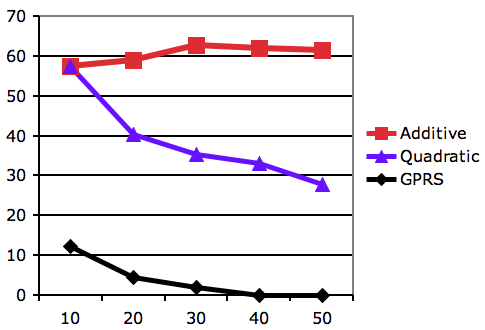
\includegraphics[scale = 0.5] {acc_sample.png} 
	\caption{ \small Comparison of model accuracy for different models as training sample size is increased.  Y-axis is average percentage error in predictions of runtime averaged across all benchmarks. X-axis is increasing sample size.  Some models are more robust to reduced sample size than others.}
	\label{fig:acc-sample}
\end{figure}